% Staircase paper for 18.821 Fall 2012 project 3.
% Authors: Daniel Grazian, Michael Mekonnen, Agustin O Venezuela III

\documentclass[12pt]{amsart}

% Keep everything here in alphabetical order, please! :) -jven

% Packages

\usepackage{amssymb}
\usepackage{graphicx}

% Enumeration

\newtheorem{theorem}{Theorem}[section]

\newtheorem{conjecture}[theorem]{Conjecture}
\newtheorem{corollary}[theorem]{Corollary}
\newtheorem{definition}[theorem]{Definition}
\newtheorem{example}[theorem]{Example}
\newtheorem{examples}[theorem]{Examples}
\newtheorem{lemma}[theorem]{Lemma}
\newtheorem{proposition}[theorem]{Proposition}
\newtheorem{remarks}[theorem]{Remarks}
\newtheorem{remark}[theorem]{Remark}

% Utility commands
% Inverse factorial
\newcommand{\ifact}{\mu}
% Determinant of our special matrix
\newcommand{\M}{M}
% Real numbers
\newcommand{\R}{\mathbb{R}}
% Figures: \newfigure{label}{caption}{content}
\newcommand{\newfigure}[3]{
\begin{figure}
#3
\caption{#2 \label{#1}}
\end{figure}
}
% Sections: \newsection{title}{label}
\newcommand{\newsection}[2]{
\section{#1 \label{#2}}
}

\title{A Staircase Model of Erosion}
\author{Daniel Grazian, Michael Mekonnen, Agustin O Venezuela III}
\date{December 10, 2012}

\begin{document}

\maketitle

\newsection{Introduction}{sec:intro}
In this paper, we consider the random process of forming staircases by dropping blocks into an infinite row of infinitely tall columns.

More concretely, consider partitioning the first quadrant of $\R^2$ into axis-aligned columns of width $1$, as in Figure $\ref{fig:columns}$. We will index the columns starting at $0$.

\newfigure{fig:columns}{Partitioning of the first quadrant into columns}{
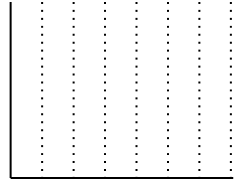
\includegraphics[scale=0.4]{columns_fig.png}
}

Now consider iteratively placing unit squares (blocks) into these columns. We will say that a block is at location $(i, j)$ for non-negative integers $i, j$ if it is axis-aligned and its bottom-left vertex is at $(i, j)$. At each step, a block can be placed at $(i, j)$ if and only if (1) $i = 0$ or there is a block at $(i - 1, j)$ and (2) $j = 0$ or there is a block at $(i, j - 1)$. Figure $\ref{fig:dropblocks}$ shows an example of a valid sequence of placing $5$ blocks. We will usually refer to such a sequence of placements a \textit{dropping of $5$ blocks}, for obvious reasons. We call a configuration of $n$ blocks in the first quadrant a \textit{staircase} if it can be obtained by dropping $n$ blocks.

\newfigure{fig:dropblocks}{Example of dropping $5$ blocks}{
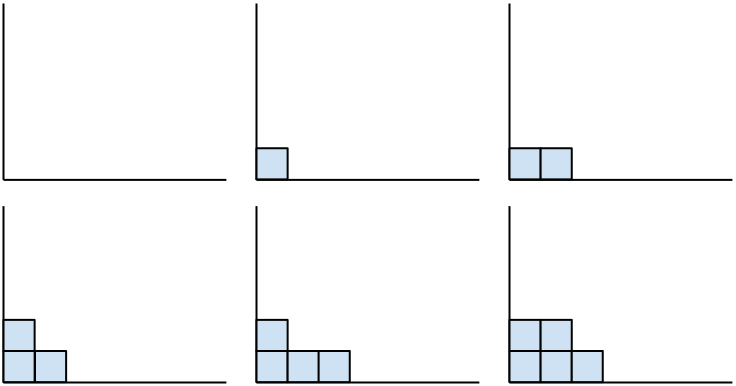
\includegraphics[scale=0.4]{dropblocks_fig.png}
}

We will refer to a staircase as the monotonically decreasing finite sequence of positive integers $(b_i)$, where $b_i$ is the number of blocks in column $i$. For example, the last staircase in Figure \ref{fig:dropblocks} can be written as $(2,2,1)$. Note that we do not include columns that do not contain any blocks.

We are interested in constructing random staircases: beginning with no blocks, we consider all the locations $(i, j)$ at which a block can be validly placed, choose such a location uniformly at random, and place a block there. This raises various interesting questions regarding the distribution over the shape of the resulting staircase when $n$ blocks are dropped.

The construction of random staircases in this manner can be likened to the process of erosion. Consider a rectangular piece of material and an eroding force acting from a fixed direction from one of its corners. If we wish to model how the shape of the material changes as a result of this force, it is reasonable to suppose that a ``piece'' of this material is not likely to be eroded unless it is exposed to the force, in the sense that it is on the surface of the material facing the direction from which the eroding force is acting. This corresponds to the process of constructing a staircase: the blocks represent the eroded pieces of material.

To begin our exposition, Section \ref{sec:numstaircases} will address the question of how many staircases exist with $n$ blocks. Section \ref{sec:numconstructions} will investigate the number of ways in which a given staircase can be formed. Section \ref{sec:twocolumn} will relate the $2$-column staircase case to the Catalan numbers and derive a well-known identity using the formula from the preceding section. Finally, Section \ref{sec:expectedcolumns} will present numerical results for the expected number of columns for a staircase with $n$ blocks.

\newsection{Number of Staircases with $n$ Blocks}{sec:numstaircases}
Our investigation into the distribution over staircase shapes begins with determining how many staircase shapes exist using $n$ blocks.

Recall that a partition of a positive integer $n$ is a sequence of monotonically decreasing positive integers whose sum is $n$.\footnote{Partition (MathWorld): http://mathworld.wolfram.com/Partition.html} Thus a staircase with $n$ blocks is equivalent to the number of partitions of $n$. For integers $n$ beginning with $n = 0$, the numbers of partitions of $n$ is $1, 1, 2, 3, 5, 7, 11, \ldots$. Unfortunately, this sequence is known to grow faster than any polynomial in $n$: for $n = 100$, there are $190,569,292$ partitions. This appears to make our original goal of finding a distribution over staircase shapes difficult as there are more than polynomially many objects to which a probability is to be assigned.

\newsection{Number of ways to construct a staircase}{sec:numconstructions}
Let us now focus on the number of ways to construct a particular staircase $(c_0, c_1, \dots, c_k)$. For instance, there are $2$ ways to construct the $(2,1)$ staircase. We begin with a few formalizing definitions, and then we proceed to developing a closed form expression for the quantity we are studying. In this section, and only in this section, we relax our formal definition of staircases by allowing $0s$ in the sequence $c_0, c_1, \dots, c_k$ to make our analysis simpler.

\begin{definition}
For a staircase $(c_0, c_1, \dots, c_k)$, let $T(c_0, c_1, \dots, c_k)$ denote the number of ways the staircase can be constructed. Let $T(c_0, \dots, c_k) = 0$ for sequences that are not staircases.
\end{definition}

We have a simple recurrence relation on $T$ that shall be useful later.

\begin{lemma}
$$\begin{array}{ccl}
T(c_0, c_1, \dots, c_k) & = & T(c_0-1, c_1, \dots, c_k) \\
& & +\ T(c_0, c_1-1, \dots, c_k) \\
& & +\ \dots \\
& & +\ T(c_0, c_1, \dots, c_k-1)
\end{array}$$
\label{lem:recurrence}
\end{lemma}

\begin{proof}
The $(c_0, c_1, \dots, c_k)$ staircase can be built in one of $k$ different ways: build the $(c_0-1, c_1, \dots, c_k)$ staircase (if possible) and then add a block to the $0^{th}$ column, or build the $(c_0, c_1-1, \dots, c_k)$ staircase (if possible) and then add a block to the $1^{st}$ column, etc. The recurrence captures exactly this idea. 
\end{proof}

\begin{definition}
For any integer $i$, we define
$$
\ifact(i) = 
\begin{cases}
\frac{1}{i!} & \text{if } i \geq 0, \\
0 & \text{otherwise.}
\end{cases}
$$
\end{definition}

To motivate the definition of $\ifact(i)$ for $i < 0$, consider the quantity $\binom{1}{-1}$. Intuitively, this quantity should be $0$ since there are $0$ ways to choose $-1$ items from a set containing $1$ item. By definition, we have that $\binom{1}{-1} = \frac{1!}{(-1)!2!}$. Thus, $\frac{1}{(-1)!} = \ifact(-1)$ ought to be $0$.

\begin{definition}
For a sequence of integers $c_0, c_1, \dots, c_k$, we define $\M(c_0, c_1, \dots, c_k)$ to be the following determinant:
$$
\M(c_0, c_1, \dots, c_k) = \left|
\begin{matrix}
\ifact(c_0) & \ifact(c_0+1) & \cdots & \ifact(c_0+k) \\
\ifact(c_1-1) & \ifact(c_1) & \cdots & \ifact(c_1+k-1) \\
\vdots & \vdots & \ddots & \vdots \\
\ifact(c_k-k) & \ifact(c_k-k+1) & \cdots & \ifact(c_k) \\
\end{matrix} \right|.
$$
\end{definition}

Here we prove a useful identity that will be useful to prove our main result.

\begin{lemma}
For a sequence of integers $c_0, c_1, \dots, c_k$, if there exists an integer $i \in \{1, 2, \dots, k\}$ such that $c_{i - 1} = c_{i} - 1$, then
$$
\M(c_0, c_1, \dots, c_k) = 0.
$$
\label{lem:mcornercase}
\end{lemma}

\begin{proof}
This result follows directly from the fact that the $(i-1)^{st}$ and $i^{th}$ rows in the determinant $\M(c_0, c_1, \dots, c_k)$ are identical.
\end{proof}

\begin{definition}
For a sequence of integers $c_0, c_1, \dots, c_k$ and an integer $i \in \{0,1,\dots,k\}$, we define $\M_i(c_0,c_1,\dots,c_k)$ to be the same as $\M(c_0, c_1, \dots, c_k)$, but with the $i^{th}$ row changed as follows:
\begin{multline*}
\M_i(c_0, c_1, \dots, c_k) = \\
\left|
\begin{matrix}
\ifact(c_0) & \ifact(c_0+1) & \cdots & \ifact(c_0+k) \\
\vdots & \vdots & \ddots & \vdots \\
-i\ifact(c_i-i) & (1-i)\ifact(c_i + 1 - i) & \cdots & (k-i) \ifact(c_i+k-i) \\
\vdots & \vdots & \ddots & \vdots \\
\ifact(c_k-k) & \ifact(c_k-k+1) & \cdots & \ifact(c_k) \\
\end{matrix} \right|.
\end{multline*}
\end{definition}

Once again, we will prove a useful identity that will be useful to prove our main result.

\begin{lemma}
For a sequence of integers $c_0, c_1, \dots, c_k$, we have
$$
\M(c_0, c_1, \dots, c_i - 1, \dots, c_k) = c_i \M(c_0, c_1, \dots, c_k) + \M_i(c_0, c_1, \dots, c_k).
$$
\label{lem:mimidentity}
\end{lemma}

\begin{proof}
$$\begin{array}{ccl}
 \M(c_0, \dots, c_i - 1, \dots, c_k) & = & \left|
\begin{matrix}
\ifact(c_0) & \cdots & \ifact(c_0+k) \\
\vdots & \ddots & \vdots \\
\ifact(c_i-i-1) & \cdots & \ifact(c_i+k-i-1) \\
\vdots & \ddots & \vdots \\
\ifact(c_k-k) & \cdots & \ifact(c_k) \\
\end{matrix} \right| \\
& = & \left|
\begin{matrix}
\ifact(c_0) & \cdots & \ifact(c_0+k) \\
\vdots & \ddots & \vdots \\
(c_i - i) \ifact(c_i-i) & \cdots & (c_i+k-i) \ifact(c_i+k-i) \\
\vdots & \ddots & \vdots \\
\ifact(c_k-k) & \cdots & \ifact(c_k) \\
\end{matrix} \right| \\
& = & c_i \M(c_0, \dots, c_i, \dots, c_k) + \M_i(c_0, \dots, c_i, \dots, c_k).
\end{array}$$
\end{proof}

\vspace{0.75cm}



Equipped with these definitions and results, we now proceed to our main result.

\begin{theorem}
For a sequence of integers $c_0 \geq c_1 \geq \dots \geq c_k \geq 0$, we have
$$
T(c_0, c_1, \dots, c_k) = (c_0 + c_1 + \dots + c_k)! \cdot \M(c_0, c_1, \dots, c_k).
$$
\label{thm:closedform}
\end{theorem}

\begin{proof}
We prove this by induction on $\sum_{i=0}^{k}{c_i}$.

In the base case, we look at $\sum_{i=0}^{k}{c_i} = 0$, where we have $c_0 = c_1 = \dots = c_k = 0$:
$$
T(0,0,\dots,0) = \M(0,0,\dots,0)=\left|
\begin{matrix}
1 & \ifact(1) & \ifact(2) & \cdots & \ifact(k) \\
0 & 1 & \ifact(1) & \cdots & \ifact(k-1) \\
0 & 0 & 1 & \cdots & \ifact(k-2) \\
\vdots & \vdots & \vdots & \ddots & \vdots \\
0 & 0 & 0 & \cdots & 1 \\
\end{matrix} \right| = 1,
$$
as desired. We get the last equality by observing that the determinant is of an upper-triangular matrix with diagonal terms that are all $1$.

In the inductive step, we assume that the theorem holds for $T(c_0-1,c_1,...,c_k)$, $T(c_0,c_1-1,...,c_k)$, $\dots$, $T(c_0,c_1,...,c_k-1)$, and show that it also holds for $T(c_0,c_1,...,c_k)$. We have to take care here since some of these cases might not respect the condition expressed in the theorem (i.e. the staircase condition). However, any of these sequences that violates the Theorem's condition satisfies the condition in Lemma \ref{lem:mcornercase}. Indeed, for these sequences, we want $T(c_0, \dots, c_i - 1, \dots, c_k) = 0$ since they violate the staircase condition. Thus, it is still safe to assume that the theorem holds for these sequences.

$$\begin{array}{ccl}
T(c_0, \dots, c_k) & = & T(c_0-1, \dots, c_k) + \dots + T(c_0, \dots, c_k-1) \\
& = & (c_0 + \dots + c_k-1)! \\
& & \cdot\ ( \M(c_0-1, \dots, c_k) + \dots + \M(c_0, \dots, c_k-1)) \\
& = & (c_0 + \dots + c_k-1)! \\
& & \cdot\ ( c_0 \M(c_0, \dots, c_k) + \M_0(c_0, c_1, \dots, c_k) \\
& & \ +\ c_1 \M(c_0, \dots, c_k) + \M_1(c_0, c_1, \dots, c_k) \\
& & \ +\ \dots \\
& & \ +\ c_k \M(c_0, \dots, c_k) + \M_k(c_0, c_1, \dots, c_k) ) \\
& = & (c_0 + \dots + c_k)! \cdot \M(c_0,\dots,c_k) \\
& & +\ (c_0+\dots+c_k-1)! \cdot (\M_0(c_0,\dots,c_k) + \dots + \M_k(c_0,\dots,c_k)).
\end{array}$$
Here we used our results from Lemmas \ref{lem:recurrence} and \ref{lem:mimidentity}.

Thus, all that remains to show now is that
\begin{equation}
\M_0(c_0,\dots,c_k) + \dots + \M_k(c_0,\dots,c_k) = 0.
\label{eqn:sumto0}
\end{equation}
Each of the summands in Equation \ref{eqn:sumto0} is a determinant of a $(k+1)\times(k+1)$ matrix, which is some linear combination of $(k+1)!$ terms. For a given permutation $(\sigma_0, \sigma_1, \dots, \sigma_k)$ of $(0,1,\dots,k)$, where $\sigma_j$ indicates the column number of the element from the $j^{th}$ row of a given matrix, the determinant $\M_i(c_0, \dots, c_k)$ contains a term of the form:
$$
C_i \prod_{j=0}^{k}{\mu(c_j+\sigma_j-j)},
$$
for some constant $C_i$. In fact, we have that $C_i = \sigma_i - i$. This follows directly from the structure of $\M_i(c_0,\dots,c_k)$. Now, we can add up all the contributions from the $k+1$ determinants to get the total constant coefficient for the term:
$$
\sum_{i=0}^{k}{C_i} = \sum_{i=0}^{k}{\sigma_i-i} = 0.
$$
Thus, we have that each of the $(k+1)!$ terms contributes nothing to the sum of determinants, giving us the result we need. Note that we have ignored the signs for these terms in the determinant computations, but this is not a problem since the signs are the same across all $k+1$ determinants.
\end{proof}

\newsection{2-Column Staircases}{sec:twocolumn}
Now we restrict ourselves to staircases of the form $(c_0,c_1)$ that have exactly $2$ columns. Using Theorem \ref{thm:closedform}, we have that
\begin{align*}
T(c_0,c_1) & = (c_0 + c_1)! \left|
\begin{matrix}
\mu(c_0) & \mu(c_0 + 1) \\
\mu(c_1 - 1) & \mu(c1)
\end{matrix}\right| \\
& =\binom{c_0 + c_1}{c_0} - \binom{c_0 + c_1}{c_1 - 1}.
\end{align*}

An interesting result we obtain is that $T(n,n) = \binom{2n}{n} - \binom{2n}{n-1}$ is exactly the $n^{th}$ Catalan number. In the $2 \times n$ rectangular $(n,n)$ staircase, we can think of the blocks in the first column as left parentheses ``(" and the blocks in the second column as right parentheses ``)". Since the staircase construction condition produces a correct parenthesization, this leads to a familiar interpretation of the Catalan numbers. 

\newsection{Expected Number of Columns}{sec:expectedcolumns}
We now consider the number of columns that occur when $n$ blocks are dropped. Our results at this point are rather minimal, but we present what we have.

There is a $\frac{1}{2^{n-1}}$ probability of a randomly constructed $n$-block staircase having one column. The only staircase of $n$ blocks with 1 column is $(n)$, a tower of $n$ blocks. The first block is guaranteed to be dropped in the first column. For $1<k \leq n$, the $k^{th}$ block is added to a staircase consisting of $(k-1)$ blocks in a single column. The $k^{th}$ block therefore has probability $\frac{1}{2}$ of being dropped in the first cloumn. So the probability of obtaining the $n$-block staircase $(n)$ is $\frac{1}{2^n}$.

Similarly, the probability of obtaining a staircase with $n$ columns is $\frac{1}{2^{n}}$. The only $n$-block staircase with $n$ columns is $(1, 1, \ldots, 1)$, and the probability of obtaining this staircase is $\frac{1}{2^{n}}$ by reasoning similar to that in the paragraph above.

However, the probability distribution of the number of columns in a randomly constructed $n$-block staircase is not symmetric. For example, for $n > 4$ it is more likely for a randomly constructed $n$-block staircase to contain $2$ columns than to contain $n-1$ columns. The only staircase with $n-1$ columns is $(2, 1, 1, \ldots, 1)$. There are $n-1$ block-dropping sequences that form this staircase, because any block after the $1^{st}$ can be the $2^{nd}$ block dropped in the $1^{st}$ column. Each of these seqences has probability less than $\frac{1}{2^{n-1}}$ of ocurring, so the probability of an $n$-block staircase having $n-1$ columns is less than $\frac{n}{2^{n-1}}$.  In contrast, there are $\lfloor \frac{n}{2} \rfloor$ staircases with $2$ columns. These are $(n-1, 1), (n-2, 2), \ldots, (\lceil \frac{n}{2} \rceil, \lfloor \frac{n}{2} \rfloor)$. The first of these staircases alone has the same probability of occurring  as the one staircase with $n-1$ columns. So the probability of a $n-1$ column staircase must be greater than that of a $2$-column staircase.

In general we suspect that the probability distribution of the number of columns in a randomly constructed staircase is strongly skewed right. Specifically, for $1 < k < \frac{n}{2}$, the probability of a staircase having $k$ columns is greater than the probability of it having $n-k+1$ columns. See figure $\ref{fig:prob_distribution}$ for the probability distribution with 50 blocks. The probability density is heavily concentrated between 6 and 20.

We also obtain a lower bound on the expectation of the number of columns in a randomly generated staircase.

\begin{theorem}
\label{lower_bound}
The expected number of blocks required for a staircase to reach $n$ columns is less than or equal to $\displaystyle\sum_{i=1}^{n}i = \frac{n(n+1)}{2}$
\end{theorem}

\begin{proof}
Consider the construction of a staircase $1$ block at a time. Given a staircase with $k-1$ columns the probability that the next block will create an extra column is greater than or equal to $\frac{1}{k}$, so the expected number of blocks required to create the next column is less than or equal to $k$. Therefore, the number of blocks required to get to the $n^{th}$ column is less than or equal to $1 + 2 + \cdots + n$. The theorem follows.
\label{thm:lower_bound}
\end{proof}

Theorem \ref{thm:lower_bound} implies that the expected number of columns in a randomly generated staircase of $\frac{n(n+1)}{2}$ blocks is greater than or equal to $n$. This means that the expected number of columns in a staircase of $n$ blocks grows at least on the order of $\sqrt{n}$.





\begin{figure}
\label{fig:prob_distribution}
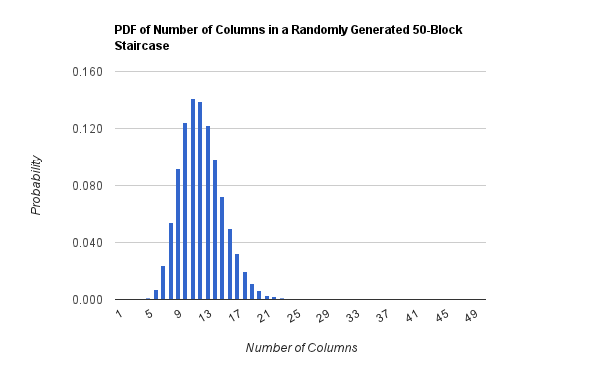
\includegraphics[scale=.75]{column_prob_chart.png}
\end{figure}
  
\newsection{Conclusion}{sec:conclusion}

This paper's main result was to enumerate the number of ways to construct a given staircase. There are other natural questions to explore in further research. For example, we showed in Section \ref{sec:expectedcolumns} that the expected number of columns in a staircase of $n$ blocks is at least on the order of $\sqrt{n}$. Further analysis might show an upper bound on the expected number of columns. Even better would be a limiting curve that the probability density function approaches as $n$ grows arbitrarily large. Another good problem would be to enumerate or bound the expected number of columns in a randomly selected staircase, without adjusting for the number of ways to construct the staircases.



\end{document}
